\chapter{Lidské oko}
\label{ch:oko}
Jedná se o~párový orgán, který nám umožňuje vnímat okolní svět a orientovat se v~prostoru pomocí světla, které se odráží od daného prostředí. Až 80 \% \cite{biofyzika} informací z~vnějšího prostředí přijímáme právě zrakem. Proto je oko nejdůležitějším smyslovým orgánem. Má přibližně kulovitý tvar a jeho stěna je rozdělena do tří vrstev: povrchová (bělima, rohovka), střední cévnatá (cévnatka, řasnaté tělísko, duhovka) a vnitřní (světločivná sítnice).

\section{Princip zrakového vjemu}
Při pohledu na nějaký předmět se světelné paprsky odrážejí od tohoto předmětu a vstupují do rohovky. Světelné paprsky jsou ohýbány a koncentrovány do jednoho místa prostřednictvím rohovky, čočky a sklivce. Z~těchto tří struktur může pouze čočka měnit svou optickou mohutnost, a tak zajišťovat, aby se paprsky koncentrovaly do místa nejostřejšího vidění. Výsledný obraz na sítnici je obrácený vzhůru nohama. Právě zde jsou světelné paprsky přeměněny na elektrické impulsy, které jsou pomocí zrakového nervu předány do mozku. Do vzpřímené polohy a výsledné podoby je obraz upraven až ve zrakovém centru v~mozku \cite{biofyzika}.

\section{Anatomie lidského oka}
Lidské oko je velmi složitý a dokonalý systém tvořený množstvím částí, které musí dokonale spolupracovat. Nejdůležitější části jsou popsány níže. Vidět je lze na obrázku \ref{pic:chap02_eye_anatomy}.

\begin{itemize}
  \item\textbf{Rohovka} je průhledná kopulovitě zakřivená vrstva pokrývající přední část oční koule. Má tvar horizontálně uložené elipsy, která se směrem dopředu vyklenuje a zabírá asi 20 \% povrchu oční koule. Je bezbarvá, zcela průhledná a bez cév. Představuje mechanickou a chemicky nepropustnou bariéru mezi vnitřním a vnějším prostředím spolu se spojivkou, sklérou a slzným filmem. Zvenku hraničí se vzduchem a směrem dovnitř je v~kontaktu s~komorovou tekutinou. Rohovka, s~ohledem na svou optickou mohutnost je nejdůležitější složkou optického systému oka a největší měrou se podílí na kvalitním vidění.
  \item\textbf{Spojivka} je tenká průsvitná tkáň, která pokrývá část vnějšího povrchu oka. Začíná na vnějším okraji rohovky, pokrývá zvnějšku viditelnou část bělimy a vystýlá také vnitřní povrch očního víčka. Je vyživována velmi tenkými cévami, které jsou prostým okem takřka neviditelné. Spojivka vylučuje hlen, který pomáhá udržovat oko vlhké.
  \item\textbf{Bělima}, též nazývaná skléra, je tuhá bílá vrstva na povrchu oční koule. Obaluje celou oční kouli kromě předního povrchu, kde přechází v~průhlednou rohovku. Ta musí být na rozdíl od bělimy prostupná pro světelné paprsky. Je velmi tuhá, a proto dobře chrání citlivé oční struktury uložené uvnitř. Na bělimu se také v~různých místech připojuje šest okohybných svalů, které umožňují pohyby očního bulbu. Na zadní straně bulbu bělimou prostupuje zrakový nerv.
  \item\textbf{Cévnatka neboli choroidea} je další vrstva obalující oční kouli, která leží mezi bělimou a sítnicí. Je velmi hustě prostoupena krevními kapilárami, kde její podstatou je vyživování oční struktury. 
  \item\textbf{Přední oční komora} je vyplněna nitrooční tekutinou a právě zde se nachází místo, odkud za normálních okolností může přebytečná tekutina odtékat. Pokud se odtok zablokuje, dochází ke zvýšení nitroočního tlaku a obvykle se rozvine i zelený zákal.
  \item\textbf{Duhovka} je barevná a neprůsvitná část nacházející se za přední komorou. Obsahuje otvor v~prostřední části, který se nazývá zornice. Průsvitnost zornice upravuje svěrač a rozšiřovač, svaly,
    které reagují na množství dopadajícího světla na sítnici.
  \item\textbf{Čočka} je důležitá pro lom světla a akomodaci, kde akomodace čočky slouží pro ostré vidění do blízka. Čočka dokáže měnit svoji optickou mohutnost, a tím i měnit index lomu světla.
  \item\textbf{Zadní oční komora} je druhou komorou nacházející se za čočkou. Taktéž obsahuje nitrooční tekutinu. Ta je za normálních okolností vylučována do zadní komory, odkud protéká do přední komory. Tam se její přebytečné množství vstřebává a odtéká z~oka pryč.
  \item\textbf{Sklivec} tvoří nejobjemnější část oka, jeho výplň. Má podobu čiré, spíše rosolovité hmoty zajišťující správný nitrooční tlak a napětí stěny oka. Naléhá na nejdůležitější a nejsložitější část oka, na sítnici.
  \item\textbf{Zrakový nerv} spojuje oko s~mozkovým zrakovým centrem. Přenáší do mozku impulsy tvořené v~sítnici. Degenerace části optického nervu je podstatou onemocnění zeleným zákalem
  \item\textbf{Sítnice} představuje nejdůležitější část této práce, proto je samostatně a podrobněji popsána v~následující sekci \ref{sec:sitnice}.
\end{itemize}

\begin{figure}[h]
  \begin{center}
    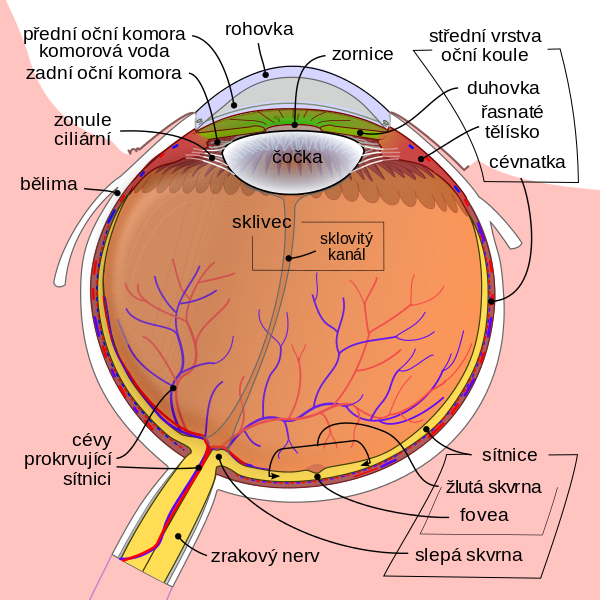
\includegraphics[width=.6\linewidth]{chap02_eye_anatomy}
    \caption{Schéma lidského oka \cite{pic_eye_anatomy}.}
    \label{pic:chap02_eye_anatomy}
  \end{center}
\end{figure}
\newpage 

\section{Sítnice}
\label{sec:sitnice}
Sítnice je nejdůležitější a také nejcitlivější částí našeho oka. Pokrývá ve formě tenké vrstvy zadní vnitřní stěnu oka. Obsahuje velké množství světločivných buněk, které umožňují vidění, a nervová vlákna. Sítnice zachycuje obraz a zrakovým nervem jej posílá do mozkové kůry. Onemocnění sítnice je vždy velmi závažné, často nevratné a může vést až ke ztrátě zraku.

\begin{itemize}
  \item\textbf{Světločivné buňky} tvoří základ fotoreceptorů. Jedná se o~buňky vytvářející nervovou stimulaci na základě absorpce fotonu přicházejícího na sítnici. Tyto buňky jsou dvojího typu: tyčinky a čípky. \textbf{Čípky} jsou citlivé na světlo různé barvy, čili různé vlnové délky, různé intenzity a různé sytosti barev. Jsou prvními neurony sítnice. Zajišťují barevné vidění za denního světla, jsou zodpovědné za zrakovou ostrost. Nacházejí se v~nejhojnějším počtu v~centrální jamce (fovea centralis) a směrem k~periferii sítnice jejich hustota postupně klesá. \textbf{Tyčinky} jsou světločivné buňky reagující na nižší intenzitu osvětlení než čípky, ale nejsou schopny rozeznávat barvy. Zajišťují noční vidění, tedy vnímání pouze jasu \cite{anatomie_oka}.
  \item\textbf{Žlutá skvrna} je struktura na sítnici představující místo nejostřejšího vidění, na kterém se tvoří obraz, když čteme nebo upřeně pozorujeme nějaký předmět. Ve svém středu obsahuje \textbf{foveu}, což je malá jamka, kde jsou nejhustěji obsaženy čípky a naopak hustota tyčinek je zde relativně malá. Z~tyčinek a čípků vycházejí nervová vlákna, která se nakonec spojují ve zrakový nerv.
  \item\textbf{Optický disk} je přibližně oválný útvar na sítnici, ve kterém vchází zrakový nerv dovnitř oční koule, tudíž neobsahuje žádné světločivné buňky. V~tomto místě se obraz netvoří, proto se také někdy nazývá slepá skvrna.
\end{itemize}

Jednotlivé části lze vidět na obrázku \ref{pic:chap02_retina}.
  
\vspace{10mm}

\begin{figure}[h]
  \begin{center}
    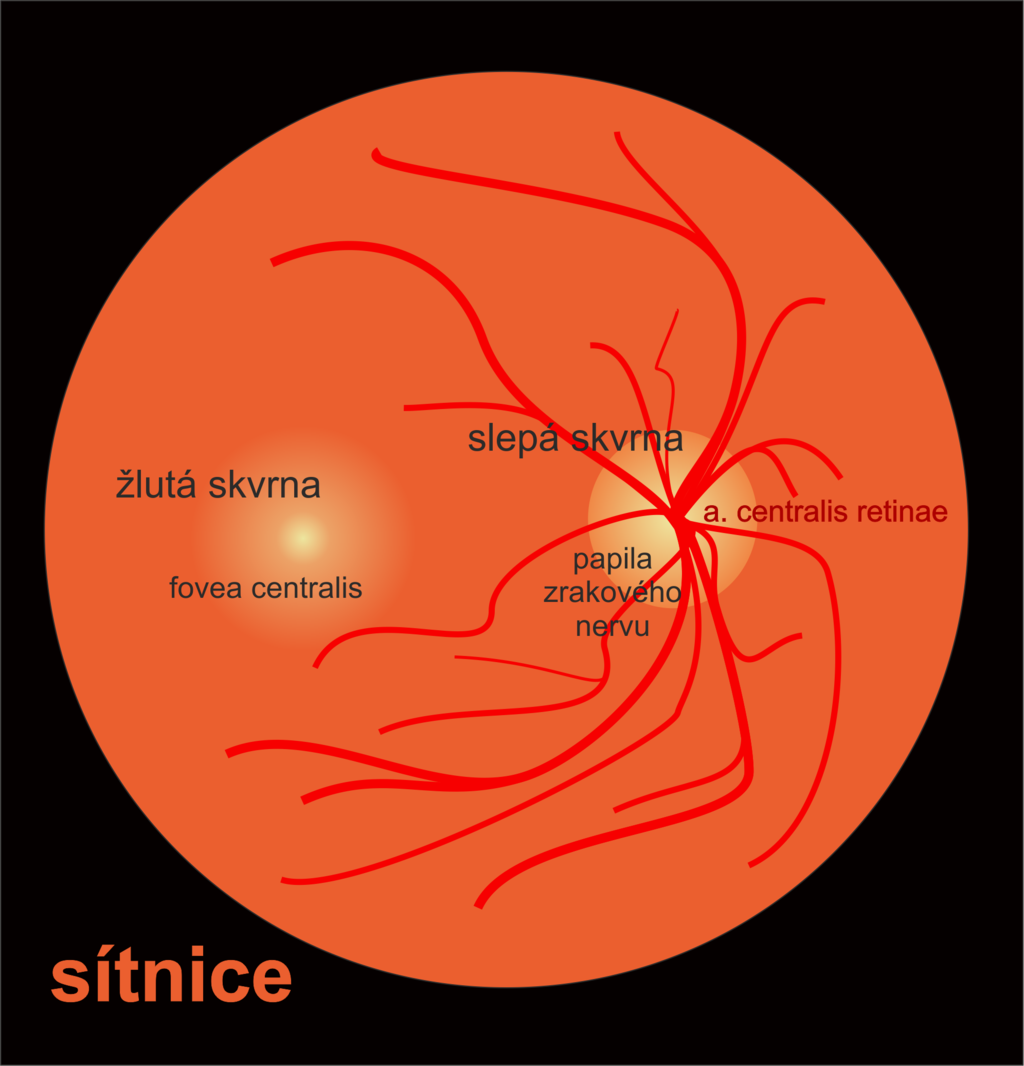
\includegraphics[width=.6\linewidth]{chap02_retina}
    \caption{Sítnice lidského oka \cite{pic_retina}.}
    \label{pic:chap02_retina}
  \end{center}
\end{figure}


\section{Vyšetření očního pozadí}
\label{sec:vysetreni}

\subsection*{Oftalmologie}
Oftalmologie je odvětví medicíny zabývající se anatomií, fyziologií, onemocněními oční bulvy a chirurgií zrakových drah, jež zahrnují oko, mozek a oblasti okolo mozku, jako je slzný systém nebo oční víčka. Jedná se o~velice úzce specializovaný obor, především vzhledem k~tomu, že oko je velmi komplikovaný aparát. Oční lékař je specialistou na lékařské a chirurgické onemocnění očí.


\subsection*{Štěrbinová lampa}
Štěrbinová lampa je nejpoužívanější přístroj v~očním lékařství. Jedná se o~speciální mikroskop, který umožňuje dokonalé vyšetření zejména předního segmentu oka: rohovky, duhovky, čočky, přední oční komory apod. Mikroskop je propojen s~lampou, jenž představuje světelný zdroj procházející úzkou štěrbinou. Lékař světlo zamíří pacientovi přímo do oka, a tak přesně nasvítí vyšetřovanou oblast. Při vyšetření jsou tkáně osvětleny buď přímým proužkem světla nebo je tkáň osvětlena zpětně odraženým světlem. Prohlížením nasvíceného oka pomocí mikroskopu pak lékař získá mnohonásobně zvětšený obraz pozorované oblasti, díky čemuž může zachytit i velmi jemné změny a příznaky očních onemocnění.

\subsection*{Oftalmoskopie}
Oftalmoskopie je vyšetření očního pozadí oftalmoskopem. Jedná se o~lékařskou pomůcku, která používá světelného paprsku, jenž je nasměrován do oka malým zrcadlem nebo hranolem a umožňuje jeho prohlédnutí. Oftalmoskopem je možné sledovat změny na cévách očního pozadí, cévnatce, sítnici i na zrakovém nervu. Rozšíření zorniček neboli mydriáza je jednoduchý a efektivní způsob, jak lze lépe pozorovat struktury za nimi. To se často provádí pomocí očních kapek před samotným vyšetřením. Existují dva hlavní typy oftalmoskopie. 

\begin{itemize}
  \item\textbf{Přímá oftalmoskopie} využívá přímého oftalmoskopu, který vytváří vzpřímený obraz přibližně 15násobného zvětšení. Jedná se o~malý přenosný nástroj, který můžete vidět na obrázku \ref{pic:chap02_ophthalmoscope_direct}. Světelný zdroj je umístěn v~horní části přístroje pod otvorem určeným pro pozorování. Sítnice se sleduje z~krátké vzdálenosti jedním okem. Tento typ oftalmoskopu se nejčastěji používá při rutinním vyšetření očního pozadí. Vyšetření se nejlépe provádí v~tmavé místnosti. Přímou oftalmoskopií lze pozorovat například degeneraci makuly. 
  \item\textbf{Nepřímé oftalmoskopie} umožňuje pozorovat větší oblasti očního pozadí v~obráceném obrazu s~2 až 5násobným zvětšením. Poskytuje širší pohled na vnitřní oko. Nepřímý oftalmoskop (obrázek \ref{pic:chap02_ophthalmoscope_indirect}) užívá speciálně upravený zdroj světla, který je umístěný na čelence, a přidaných čoček lupy, které jsou kladeny do blízkosti oka. To umožňuje vyšetření sítnice z~větší vzdálenosti. Nepřímý oftalmoskop poskytuje silnější světelný zdroj, speciálně konstruovaný objektiv a možnost stereoskopické kontroly vnitřku oční bulvy. Zornice musí být plně rozšířeny pro uspokojivý výsledek. Používá se k~perifernímu sledování sítnice pro pozorování nitroočních zánětů, u~cévních mozkových příhod, roztroušené sklerózy, nitrolební hypertenze aj.
\end{itemize}

\begin{figure}[h]
  \begin{minipage}[c]{0.47\textwidth}
    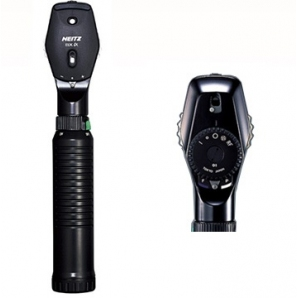
\includegraphics[width=\linewidth]{chap02_ophthalmoscope_direct}
    \caption{Přímý oftalmoskop \cite{pic_dir_scope}.}
    \label{pic:chap02_ophthalmoscope_direct}
  \end{minipage}
  \hfill
  \begin{minipage}[c]{0.47\textwidth}
    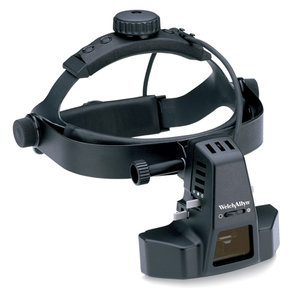
\includegraphics[width=\linewidth]{chap02_ophthalmoscope_indirect}
    \caption{Nepřímý oftalmoskop \cite{pic_indir_scope}.}
    \label{pic:chap02_ophthalmoscope_indirect}
  \end{minipage}
\end{figure}
  

\subsection*{Fundus kamera}
Fundus kamera (obrázek \ref{pic:chap02_fundus_camera}) je přístroj nahrazující oftalmoskop. Je založena na principu monokulární nepřímé oftalmoskopie. Fundus kamera poskytuje vzpřímený, zvětšený záběr na oční pozadí. Typická kamera zobrazuje 30 až 50$^\circ$ oblasti sítnice se zvětšením 2,5$\times$ a umožňuje změnu tohoto vztahu pomocí zoomu nebo pomocných čoček. Optika fundus kamery je podobná optice nepřímého oftalmoskopu v~tom, že pozorovací a osvětlovací systémy následují odlišné cesty. Jejím výstupem jsou digitální obrazy sítnice, které se používají pro sledování stavu sítnice a případnou diagnostiku očních onemocnění. Použití této kamery je neinvazivní, tedy nijak nezasahuje do snímaného oka. Před vyšetřením se aplikují oční kapky na rozšíření zornic \cite{pristroje}.

\begin{figure}[h]
  \begin{center}
    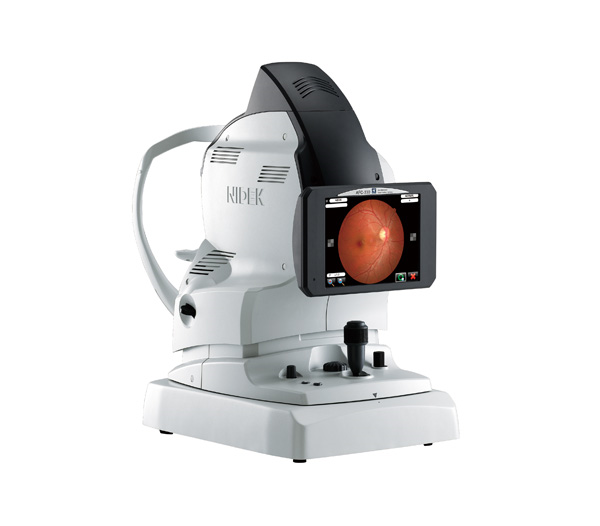
\includegraphics[width=0.7\linewidth]{chap02_fundus_camera}
    \caption{Fundus kamera \cite{pic_fundus}.}
    \label{pic:chap02_fundus_camera}
  \end{center}
\end{figure}